% ============================================================
%  INFORME TÉCNICO -- INFORME 1.1
%  Configuración e Instalación del SDK de Flutter
%  Universidad de las Fuerzas Armadas ESPE
%  Desarrollo de Aplicaciones Móviles -- NRC 30738
% ============================================================
\documentclass[12pt,a4paper]{article}

% --- Codificación y lengua --------------------------------
\usepackage[utf8]{inputenc}
\usepackage[T1]{fontenc}
\usepackage[spanish,es-noindentfirst]{babel}

% --- Márgenes ------------------------------------------
\usepackage{geometry}
\geometry{top=2.5cm, bottom=2.5cm, left=3cm, right=2.5cm}

% --- Tipografía y espaciado ----------------------------
\usepackage{lmodern}
\usepackage{microtype}
\usepackage{setspace}
\setstretch{1.5}
\usepackage{parskip}
\setlength{\parindent}{0pt}

% --- Gráficos ------------------------------------------
\usepackage{graphicx}
\usepackage{float}
\newfloat{anexofloat}{H}{loax}
\floatname{anexofloat}{Anexo}
\usepackage{caption}
\usepackage{subcaption}

% --- Encabezados/pies ----------------------------------
\usepackage{fancyhdr}
\setlength{\headheight}{78.33pt}
\addtolength{\topmargin}{-64.33pt}
\pagestyle{fancy}
\fancyhf{}
\fancyhead[L]{\small\textcolor{espeblue}{ESPE -- Desarrollo de Aplicaciones Móviles}}
\fancyhead[R]{\small\textcolor{espeblue}{NRC: 30738}}
\fancyfoot[C]{\thepage}
\renewcommand{\headrulewidth}{0.4pt}

% Estilo para la portada (logo centrado, sin línea)
\fancypagestyle{portada}{%
  \fancyhf{}
  \fancyhead[C]{
\includegraphics[height=2.6cm]{espe.png}}
  \renewcommand{\headrulewidth}{0pt}
}

% --- Colores -------------------------------------------
\usepackage{xcolor}
\definecolor{espeblue}{RGB}{0,51,102}
\definecolor{codegray}{rgb}{0.5,0.5,0.5}
\definecolor{codepurple}{rgb}{0.58,0,0.82}
\definecolor{backcolour}{rgb}{0.95,0.95,0.92}
\definecolor{dartblue}{RGB}{84,176,220}
\definecolor{androidgreen}{RGB}{61,220,132}

% --- Secciones -----------------------------------------
\usepackage{titlesec}
\titleformat{\section}{\large\bfseries\color{espeblue}}{\thesection.}{0.5em}{}[\color{espeblue}\titlerule]
\titleformat{\subsection}{\normalsize\bfseries\color{espeblue!80}}{\thesubsection}{0.5em}{}
\titleformat{\subsubsection}{\normalsize\itshape\color{espeblue!70}}{\thesubsubsection}{0.5em}{}

% --- Tabla de contenidos -------------------------------
\usepackage{tocloft}
\renewcommand{\cftsecleader}{\cftdotfill{\cftdotsep}}
\renewcommand{\cftsubsecleader}{\cftdotfill{\cftdotsep}}

% --- Tablas -------------------------------------------
\usepackage{booktabs}
\usepackage{array}

% --- Matemáticas --------------------------------------
\usepackage{amsmath}
\usepackage{amssymb}

% --- TikZ para diagramas de arquitectura -------------
\usepackage{tikz}
\usetikzlibrary{shapes.geometric, shapes.misc, arrows.meta, positioning, calc, fit, backgrounds}

\tikzset{
  compbox/.style={
    rectangle, rounded corners=5pt,
    draw=#1!70!black, fill=#1!15,
    minimum width=5.0cm, minimum height=0.95cm,
    align=center, text width=4.8cm, font=\small\bfseries, text=#1!60!black
  },
  subbox/.style={
    rectangle, rounded corners=2pt,
    draw=#1!60!black, fill=#1!8,
    minimum width=4.2cm, minimum height=0.72cm,
    text centered, font=\footnotesize
  },
  arrow/.style={thick, -Stealth, color=espeblue},
  darrow/.style={thick, Stealth-Stealth, color=espeblue!60, dashed},
}

% --- Código fuente / comandos shell ------------------
\usepackage{listings}
\lstdefinestyle{shellStyle}{
  backgroundcolor=\color{backcolour},
  basicstyle=\ttfamily\footnotesize,
  breaklines=true,
  frame=single,
  rulecolor=\color{espeblue!40},
  numbers=none,
  captionpos=b,
}
\lstset{style=shellStyle}

% --- Hipervínculos ------------------------------------
\usepackage{hyperref}
\hypersetup{
  colorlinks=true,
  linkcolor=espeblue,
  citecolor=espeblue,
  urlcolor=dartblue,
  pdftitle={Informe 2.1 - Desarrollo de Calculadora en FlutterFlow - ESPE},
}

% ============================================================
\begin{document}
% ============================================================

% ============================================================
%  PORTADA
% ============================================================
\thispagestyle{portada}
\singlespacing
\setlength{\parskip}{0pt}
\vspace*{1.2cm}
\begin{center}
  {\Large\bfseries\color{espeblue}
    UNIVERSIDAD DE LAS FUERZAS ARMADAS ESPE\\[0.3cm]}
  {\large\color{espeblue}
    Departamento de Ciencias de la Computación\\[0.2cm]
    Asignatura: Desarrollo de Aplicaciones Móviles\\[0.2cm]
    NRC: 30738\\[0.6cm]}
  \textcolor{espeblue}{\rule{\linewidth}{1.5pt}}\\[0.4cm]
  {\LARGE\bfseries\color{espeblue}
    Informe 2.1\\[0.25cm]
    Desarrollo de Calculadora Funcional en FlutterFlow\\[0.35cm]}
  \textcolor{espeblue}{\rule{\linewidth}{1.5pt}}\\[1.0cm]
  {\large\bfseries Integrantes:}\\[0.4cm]
  \begin{tabular}{c}
    Arroyo Alfonso\\[0.15cm]
    Cáceres Germán\\[0.15cm]
    Frías Pedro\\[0.15cm]
    Llumiquinga Ariel\\
  \end{tabular}\\[1.5cm]
  {\large\textbf{Docente:} Ing. Doris Chicacza MSc}\\[0.35cm]
  {\large\textbf{Fecha:} 19 de mayo de 2026}\\[0.35cm]
  
  {\large\textbf{Link Entregables:}}\\[0.35cm]
  {\large\url{https://github.com/Gpcaceres/grupo-moviles-poryectos.git}}\\[0.35cm]
\end{center}


\newpage
\pagenumbering{roman}

% ============================================================
%  ÍNDICES
% ============================================================
\tableofcontents

\listoffigures

\listof{anexofloat}{Índice de Anexos}
\addcontentsline{toc}{section}{Índice de Anexos}

\newpage
\pagenumbering{arabic}
\setcounter{page}{1}

% ============================================================
%  1. INTRODUCCIÓN
% ============================================================
\section{Introducción}

El desarrollo de aplicaciones móviles ha experimentado una transformación significativa con la aparición de plataformas de desarrollo visual y \textit{low-code}. \textbf{FlutterFlow}, lanzado en 2020, se ha consolidado como una de las herramientas más potentes en este paradigma, permitiendo crear aplicaciones Flutter completamente funcionales mediante una interfaz gráfica de arrastrar y soltar (\textit{drag-and-drop}), sin necesidad de escribir código manual~\cite{flutterflow2024}.

Este informe documenta el proceso de desarrollo de una \textbf{calculadora funcional} en FlutterFlow, implementando las cuatro operaciones aritméticas básicas (suma, resta, multiplicación y división). El proyecto integra componentes visuales (\textit{widgets}), variables de estado (\textit{Page State}) y flujos de acciones (\textit{Action Flow Editor}) para demostrar la capacidad de FlutterFlow de gestionar lógica de negocio compleja mediante configuración visual.

\subsection{Objetivos}

\subsubsection{Objetivo General}

Desarrollar una aplicación de calculadora funcional en FlutterFlow que implemente operaciones aritméticas básicas mediante la configuración visual de componentes, variables de estado y flujos de acciones.

\subsubsection{Objetivos Específicos}

\begin{itemize}
  \item Diseñar la interfaz de usuario con campos de entrada numéricos y botones de operación.
  \item Implementar una variable de estado tipo \texttt{Double} para almacenar y mostrar resultados.
  \item Configurar flujos de acciones (\textit{Action Flows}) para cada operación aritmética.
  \item Utilizar expresiones personalizadas (\textit{Inline Functions}) para ejecutar operaciones matemáticas.
  \item Validar el funcionamiento de la calculadora mediante pruebas de las cuatro operaciones básicas.
\end{itemize}

% ============================================================
%  2. MARCO TEÓRICO
% ============================================================
\section{Marco Teórico}

\subsection{FlutterFlow}

\textbf{FlutterFlow} es una plataforma de desarrollo visual \textit{low-code} creada por ex-ingenieros de Google, lanzada oficialmente en 2020. Permite diseñar, construir y desplegar aplicaciones Flutter completas sin necesidad de escribir código manualmente, mediante una interfaz de arrastrar y soltar~\cite{flutterflow2024}. A diferencia de otros constructores visuales que generan código propietario o difícil de mantener, FlutterFlow produce código Flutter estándar y limpio que puede exportarse, modificarse y mantenerse en cualquier IDE tradicional~\cite{lowcode2023}.

Las características principales de FlutterFlow incluyen:

\begin{itemize}
  \item \textbf{Editor visual de UI}: construcción de interfaces mediante \textit{widgets} de Flutter arrastrables.
  \item \textbf{Sistema de navegación}: configuración visual de rutas y transiciones entre páginas.
  \item \textbf{Gestión de estado}: variables de ámbito de aplicación (\textit{App State}) y de página (\textit{Page State}).
  \item \textbf{Action Flow Editor}: editor visual de lógica de negocio sin código.
  \item \textbf{Integraciones nativas}: conexión con Firebase, Supabase, APIs REST y servicios externos.
  \item \textbf{Exportación de código}: descarga del proyecto Flutter completo para desarrollo híbrido~\cite{flutterflow2024}.
\end{itemize}

\subsection{Paradigma Low-Code}

Las plataformas \textit{low-code} permiten desarrollar aplicaciones completas mediante configuración visual, reduciendo drásticamente la cantidad de código escrito manualmente. Según Gartner, se estima que para 2026 más del 65\% del desarrollo de aplicaciones empresariales se realizará mediante plataformas \textit{low-code} o \textit{no-code}~\cite{gartner2023}. Este paradigma democratiza el desarrollo de software, permitiendo que diseñadores, analistas de negocio y desarrolladores colaboren en un mismo entorno visual~\cite{lowcode2023}.

FlutterFlow se clasifica como \textit{low-code} porque, aunque la mayor parte del desarrollo es visual, permite insertar código Dart personalizado mediante \textit{Custom Functions} y \textit{Custom Actions} cuando se requiere lógica compleja no soportada nativamente~\cite{flutterflow2024}.

\subsection{Gestión de Estado en FlutterFlow}

El \textbf{estado} de una aplicación representa los datos que cambian a lo largo del tiempo (valores de formularios, resultados de cálculos, datos descargados de APIs, etc.). FlutterFlow implementa dos niveles de estado~\cite{flutterflow2024}:

\begin{itemize}
  \item \textbf{App State}: variables globales accesibles desde cualquier página de la aplicación. Persisten durante toda la sesión del usuario.
  \item \textbf{Page State}: variables locales a una página específica. Se destruyen al salir de la página y se recrean al entrar nuevamente.
\end{itemize}

Cada variable de estado tiene un tipo de dato definido (\texttt{String}, \texttt{Integer}, \texttt{Double}, \texttt{Boolean}, \texttt{List}, etc.) y puede tener un valor inicial. Los \textit{widgets} pueden ``escuchar'' estas variables y actualizarse automáticamente cuando cambian, implementando el patrón reactivo de Flutter~\cite{flutter2024}.

\subsection{Action Flow Editor}

El \textbf{Action Flow Editor} es el editor visual de lógica de FlutterFlow. Permite configurar secuencias de acciones que se ejecutan en respuesta a eventos de usuario (clics, deslizamientos, envíos de formularios, etc.)~\cite{flutterflow2024}. Las acciones disponibles incluyen:

\begin{itemize}
  \item \textbf{Navegación}: abrir páginas, regresar, abrir diálogos.
  \item \textbf{Actualización de estado}: modificar variables de \textit{App State} o \textit{Page State}.
  \item \textbf{Lógica condicional}: ejecutar acciones solo si se cumple una condición.
  \item \textbf{Operaciones de backend}: llamadas a APIs, consultas a Firebase, autenticación.
  \item \textbf{Funciones personalizadas}: ejecutar código Dart mediante \textit{Inline Functions} o \textit{Custom Actions}.
\end{itemize}

El \textit{Action Flow Editor} estructura las acciones en un flujo visual, permitiendo encadenar múltiples pasos de forma secuencial o condicional, facilitando la comprensión y el mantenimiento de la lógica de negocio sin necesidad de leer código~\cite{flutterflow2024}.

\subsection{Inline Functions y Code Expressions}

Cuando la lógica requerida no puede configurarse completamente con acciones visuales, FlutterFlow permite insertar \textbf{expresiones de código Dart} directamente en el flujo de acciones. Estas expresiones, llamadas \textit{Inline Functions} o \textit{Code Expressions}, reciben variables de entrada (\texttt{var1}, \texttt{var2}, etc.) y retornan un valor calculado~\cite{flutterflow2024}.

Por ejemplo, para dividir dos números capturados desde campos de texto, se utiliza la expresión:

\begin{lstlisting}[caption={Expresión Dart para división en FlutterFlow}]
var1 / var2
\end{lstlisting}

Esta capacidad permite implementar lógica matemática, manipulación de cadenas, conversiones de datos y validaciones personalizadas sin abandonar el editor visual~\cite{flutterflow2024}.

% ============================================================
%  3. ARQUITECTURA DE LA CALCULADORA
% ============================================================
\section{Arquitectura de la Calculadora en FlutterFlow}

La figura~\ref{fig:arquitectura} ilustra la arquitectura de componentes de la calculadora desarrollada en FlutterFlow. El flujo de datos comienza con la captura de valores numéricos desde los campos de entrada, pasa por el procesamiento mediante \textit{Inline Functions} ejecutadas desde los botones de operación, y finaliza con la actualización de la variable de estado \texttt{result} que alimenta el widget de visualización.

\begin{figure}[H]
\centering
\begin{tikzpicture}[node distance=1.1cm]

  % --- Fila superior: Campos de entrada ---
  \node (input1) [compbox=espeblue] {Campo de Entrada 1\\[2pt]{\footnotesize \texttt{inputNum1} -- tipo Number}};
  \node (input2) [compbox=espeblue, right=0.8cm of input1] {Campo de Entrada 2\\[2pt]{\footnotesize \texttt{inputNum2} -- tipo Number}};

  % --- Fila intermedia: Botones de operación ---
  \node (buttons) [compbox=dartblue, below=1.2cm of input1, minimum width=11cm, xshift=2.9cm]
        {Botones de Operación\\[2pt]{\footnotesize $+$ / $-$ / $\times$ / $\div$}};

  % --- Fila de procesamiento: Inline Function ---
  \node (inline) [compbox=androidgreen, below=1.2cm of buttons]
        {Inline Function (Code Expression)\\[2pt]{\footnotesize \texttt{var1 [operador] var2}}};

  % --- Fila de estado: Page State Variable ---
  \node (state) [compbox=orange, below=1.2cm of inline]
        {Variable de Estado (Page State)\\[2pt]{\footnotesize \texttt{result} -- tipo Double}};

  % --- Fila inferior: Widget de visualización ---
  \node (display) [compbox=red!70!black, below=1.2cm of state]
        {Widget de Visualización (Text)\\[2pt]{\footnotesize Muestra el valor de \texttt{result}}};

  % --- Flechas del flujo de datos ---
  \draw[arrow] (input1.south) -- ++(0,-0.4) -| (buttons.north -| input1.south);
  \draw[arrow] (input2.south) -- ++(0,-0.4) -| (buttons.north -| input2.south);
  \draw[arrow] (buttons) -- node[right, font=\footnotesize]{On Tap Action} (inline);
  \draw[arrow] (inline) -- node[right, font=\footnotesize]{retorna valor} (state);
  \draw[arrow] (state) -- node[right, font=\footnotesize]{actualiza} (display);

  % --- Anotación lateral ---
  \node[text width=3.5cm, font=\footnotesize, right=0.5cm of inline, anchor=west]
        {Cada botón ejecuta un \textit{Action Flow} que lee los campos, calcula y actualiza \texttt{result}};

\end{tikzpicture}
\caption{Arquitectura de flujo de datos de la calculadora en FlutterFlow}
\label{fig:arquitectura}
\end{figure}

El espacio de trabajo de FlutterFlow (figura~\ref{fig:workspace}) muestra la interfaz completa del editor visual, incluyendo el árbol de \textit{widgets} a la izquierda, el lienzo de diseño al centro y el panel de propiedades a la derecha.

\begin{figure}[H]
  \centering
  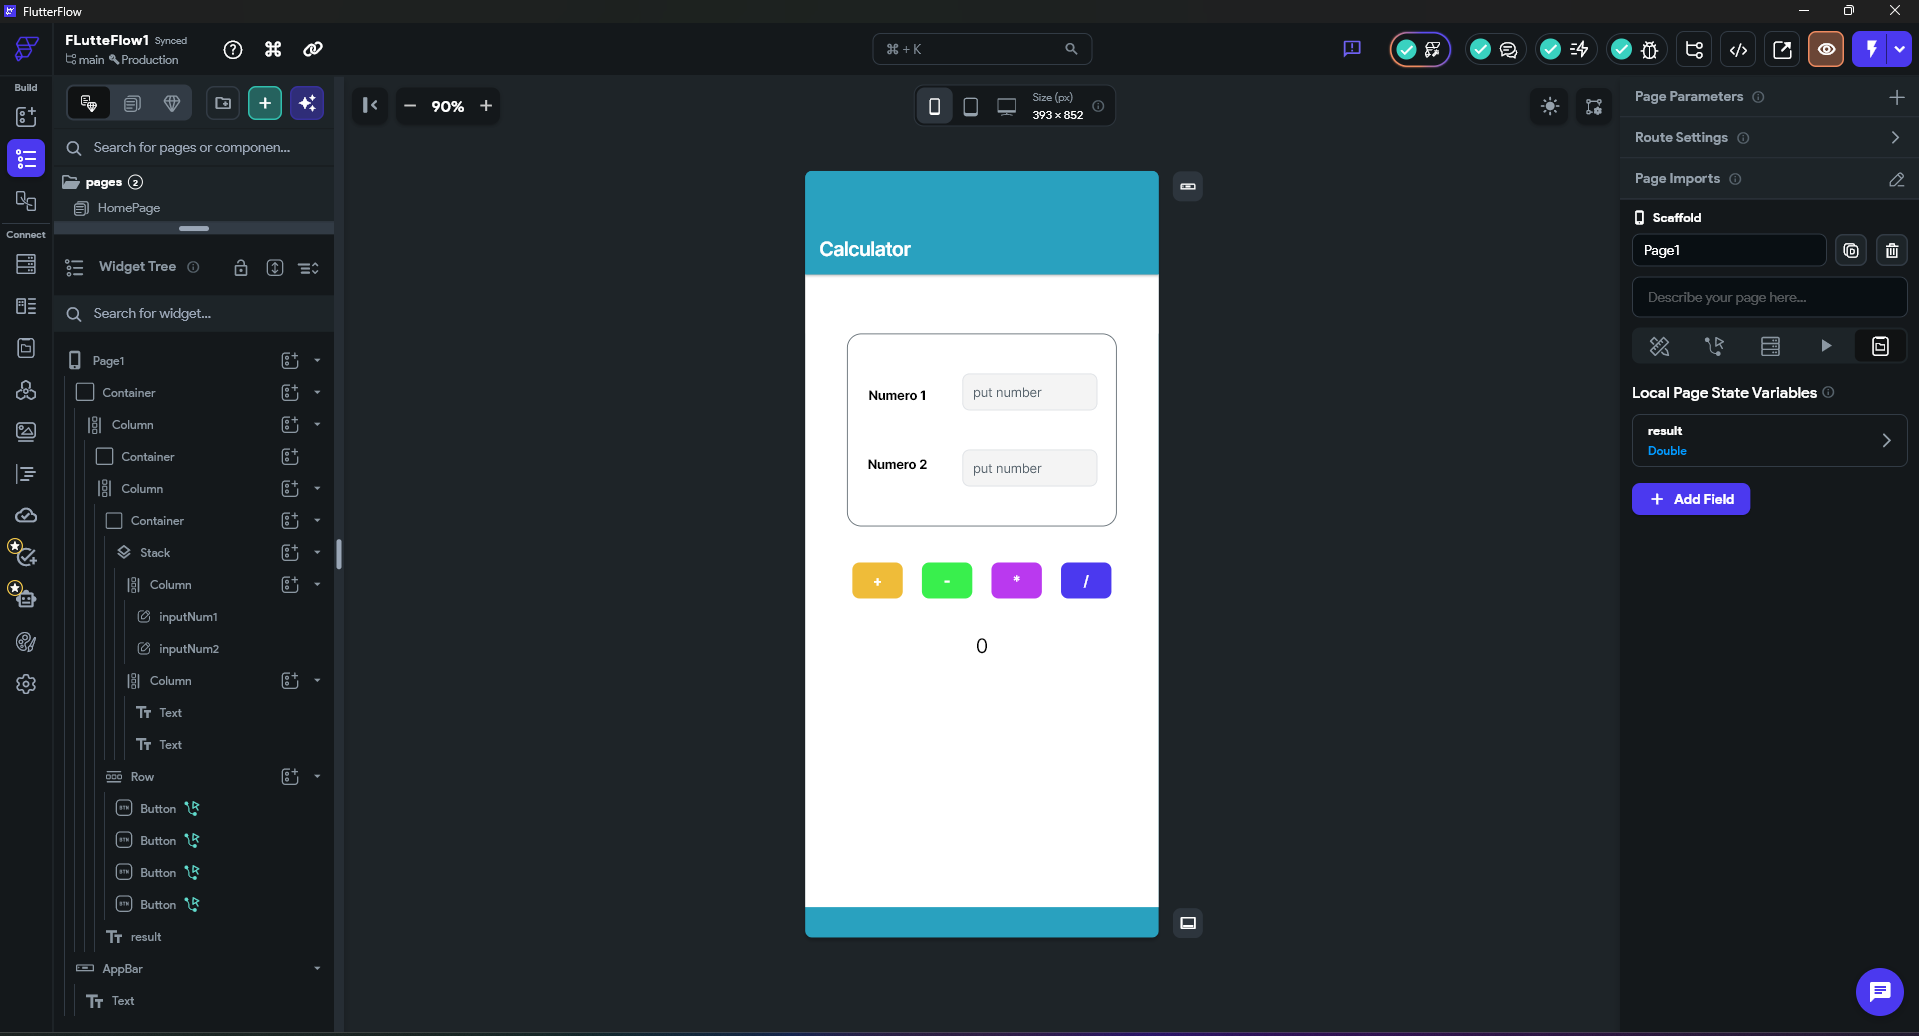
\includegraphics[width=0.95\textwidth]{img/EspacioDeTRabajoFlutterFlow.png}
  \caption{Espacio de trabajo de FlutterFlow -- vista del editor visual}
  \label{fig:workspace}
\end{figure}

% ============================================================
%  4. PROCEDIMIENTO DE DESARROLLO
% ============================================================
\section{Procedimiento de Desarrollo}

\subsection{Paso 1 -- Diseño de la Interfaz de Usuario}

La interfaz de la calculadora se construyó utilizando los siguientes componentes de FlutterFlow:

\begin{itemize}
  \item \textbf{Container}: contenedor principal que agrupa todos los elementos visuales.
  \item \textbf{Column}: organiza los elementos verticalmente (campos de entrada, botones, resultado).
  \item \textbf{TextField}: dos campos de entrada configurados para aceptar únicamente valores numéricos (\texttt{inputNum1} e \texttt{inputNum2}).
  \item \textbf{Row}: organiza los cuatro botones de operación horizontalmente.
  \item \textbf{Button}: cuatro botones ($+$, $-$, $\times$, $\div$) con colores diferenciados.
  \item \textbf{Text}: widget de visualización del resultado en la parte inferior.
\end{itemize}
\newpage
La figura~\ref{fig:componentes} muestra la jerarquía de \textit{widgets} utilizada en el proyecto.

\begin{figure}[H]
  \centering
  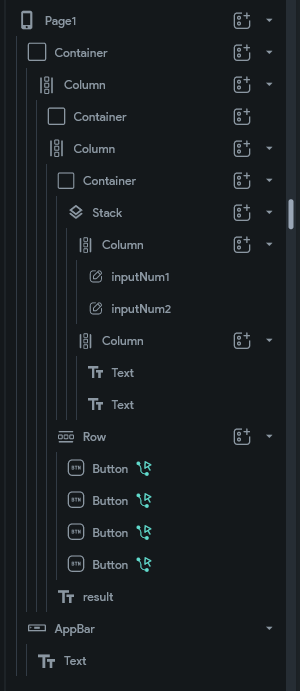
\includegraphics[width=0.35\textwidth]{img/componentesUsadosFlutterFlow.png}
  \caption{Árbol de componentes (\textit{Widget Tree}) de la calculadora}
  \label{fig:componentes}
\end{figure}

Los campos de entrada fueron configurados con las siguientes propiedades:
\begin{itemize}
  \item \texttt{Keyboard Type}: \textit{Number} (solo permite dígitos y punto decimal).
  \item \texttt{Hint Text}: ``put number'' (texto de ayuda).
  \item \texttt{Controller Name}: \texttt{inputNum1} e \texttt{inputNum2} para referencia posterior.
\end{itemize}

\subsection{Paso 2 -- Creación de la Variable de Estado}

Para almacenar el resultado de las operaciones, se creó una variable de tipo \textbf{Page State} con las siguientes características:

\begin{itemize}
  \item \textbf{Nombre}: \texttt{result}
  \item \textbf{Tipo}: \texttt{Double}
  \item \textbf{Valor inicial}: \texttt{0}
  \item \textbf{Ámbito}: \textit{Page State} (local a la página de la calculadora)
\end{itemize}

Las variables de \textit{Page State} permiten que los \textit{widgets} reaccionen automáticamente a cambios de valor. En este caso, el widget \texttt{Text} del resultado está vinculado a la variable \texttt{result}, actualizándose visualmente cada vez que esta cambia (figura~\ref{fig:variableResult}).

\begin{figure}[H]
  \centering
  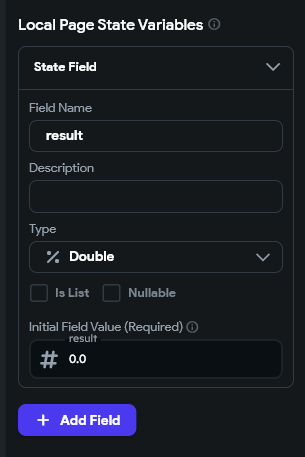
\includegraphics[width=0.35\textwidth]{img/creacioVariableResult.png}
  \caption{Configuración de la variable de estado \texttt{result} (tipo Double)}
  \label{fig:variableResult}
\end{figure}

\subsection{Paso 3 -- Configuración del Action Flow para las Operaciones}

Cada botón de operación ($+$, $-$, $\times$, $\div$) ejecuta un \textbf{Action Flow} al ser presionado (evento \texttt{On Tap}). El flujo de acciones sigue la siguiente secuencia:

\begin{enumerate}
  \item \textbf{Lectura de Valores}: se extraen los valores numéricos actuales de \texttt{inputNum1} e \texttt{inputNum2}.
  \item \textbf{Ejecución de Operación}: se utiliza una \textit{Inline Function} para realizar el cálculo matemático correspondiente.
  \item \textbf{Actualización de Estado}: el resultado se almacena en la variable \texttt{result} mediante la acción \texttt{Update Page State}.
  \item \textbf{Reconstrucción del Widget}: el widget \texttt{Text} vinculado a \texttt{result} se redibuja automáticamente con el nuevo valor.
\end{enumerate}

La figura~\ref{fig:actionFlow} muestra la configuración del \textit{Action Flow Editor} para el botón de división, incluyendo la asignación de las dos variables de entrada (\texttt{var1} y \texttt{var2}) y la expresión Dart \texttt{var1 / var2}.

\begin{figure}[H]
  \centering
  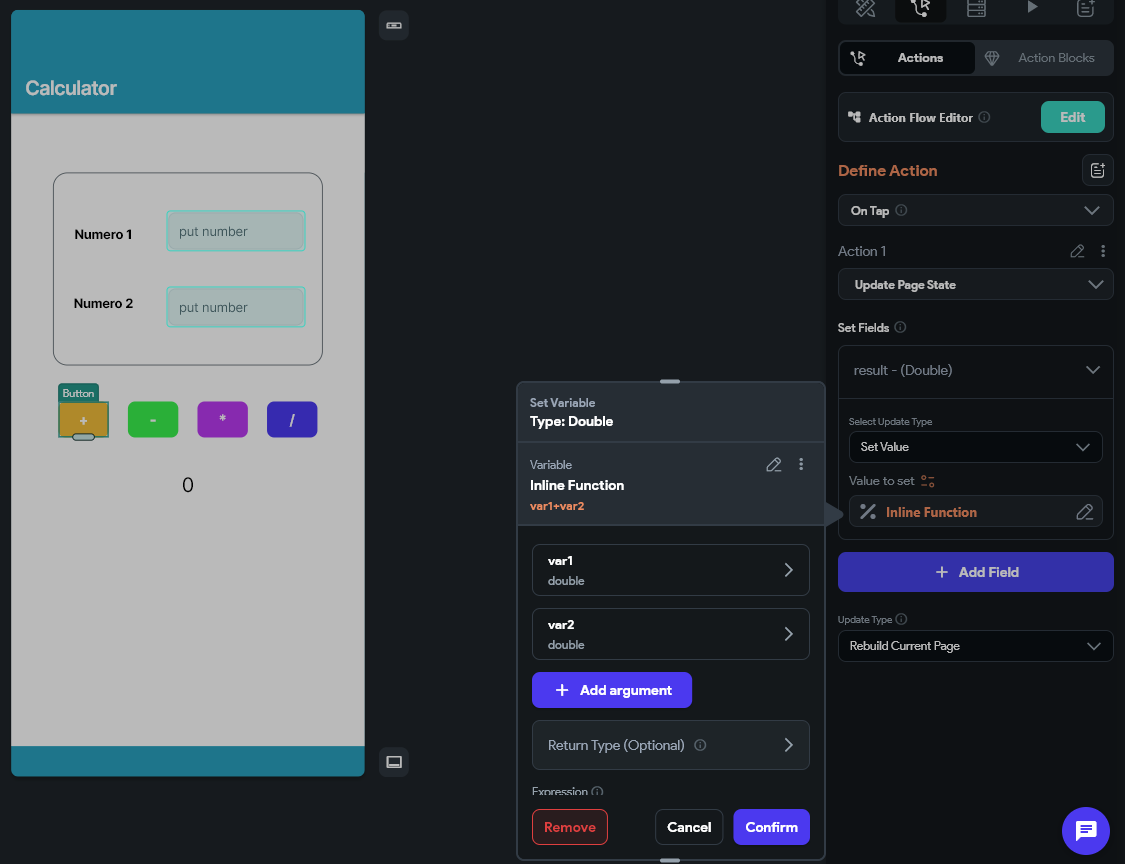
\includegraphics[width=0.85\textwidth]{img/asignacionVariabeResultEveryButton.png}
  \caption{Configuración del \textit{Action Flow} -- asignación de variables y operación}
  \label{fig:actionFlow}
\end{figure}

\subsection{Paso 4 -- Implementación de Inline Functions}

Para cada operación aritmética se configuró una \textbf{Inline Function} con los siguientes parámetros:

\begin{itemize}
  \item \textbf{Variables de entrada}:
    \begin{itemize}
      \item \texttt{var1} (tipo \texttt{double}): valor del primer campo de entrada.
      \item \texttt{var2} (tipo \texttt{double}): valor del segundo campo de entrada.
    \end{itemize}
  \item \textbf{Tipo de retorno}: \texttt{double}
  \item \textbf{Expresión de código}:
    \begin{itemize}
      \item \textbf{Suma}: \texttt{var1 + var2}
      \item \textbf{Resta}: \texttt{var1 - var2}
      \item \textbf{Multiplicación}: \texttt{var1 * var2}
      \item \textbf{División}: \texttt{var1 / var2}
    \end{itemize}
\end{itemize}

Estas funciones se ejecutan en tiempo real al presionar cada botón, calculan el resultado y lo retornan a la acción \texttt{Update Page State} que actualiza la variable \texttt{result}.

\subsection{Paso 5 -- Pruebas de Funcionalidad}

Se realizaron pruebas de cada operación con diferentes valores de entrada para validar el correcto funcionamiento de la calculadora. Las figuras~\ref{fig:suma} a~\ref{fig:division} muestran los resultados de las pruebas realizadas con los valores de ejemplo 7 y 9.

% ============================================================
%  5. ANÁLISIS DE RESULTADOS
% ============================================================
\section{Análisis de Resultados}

La calculadora desarrollada en FlutterFlow demostró funcionar correctamente para las cuatro operaciones aritméticas básicas. Se realizaron pruebas con los valores de entrada \textbf{7} y \textbf{9}, obteniendo los resultados esperados en cada caso.

\subsection{Resultados de las Operaciones}

\begin{figure}[H]
  \centering
  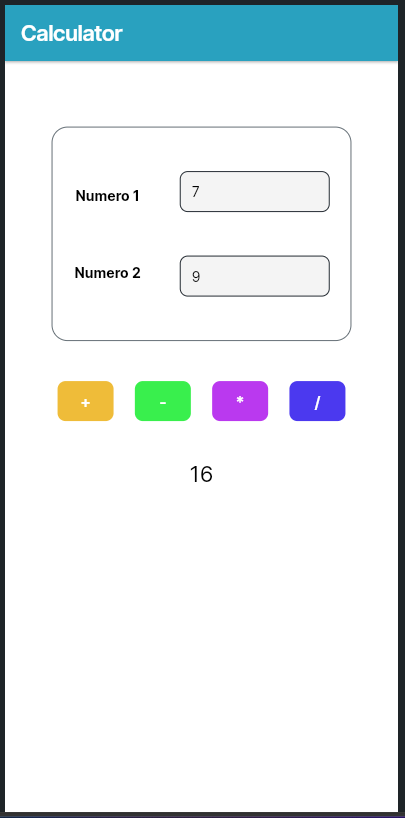
\includegraphics[width=0.25\textwidth]{img/suma.png}
  \caption{Resultado de la suma: $7 + 9 = 16$}
  \label{fig:suma}
\end{figure}

\begin{figure}[H]
  \centering
  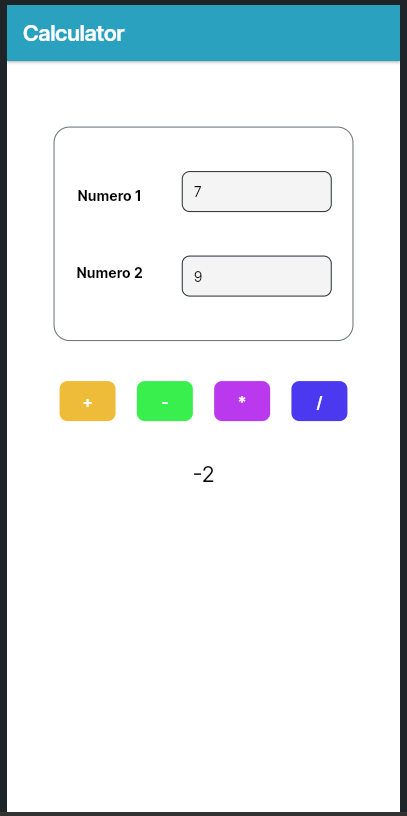
\includegraphics[width=0.25\textwidth]{img/resta.png}
  \caption{Resultado de la resta: $7 - 9 = -2$}
  \label{fig:resta}
\end{figure}

\begin{figure}[H]
  \centering
  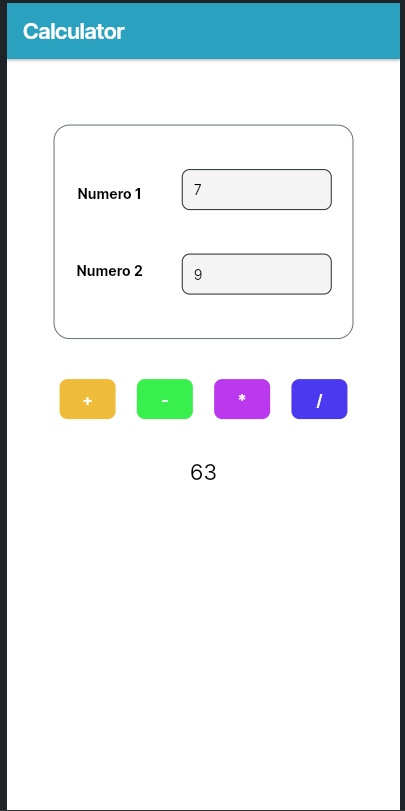
\includegraphics[width=0.25\textwidth]{img/multiplicacion.png}
  \caption{Resultado de la multiplicación: $7 \times 9 = 63$}
  \label{fig:multiplicacion}
\end{figure}

\begin{figure}[H]
  \centering
  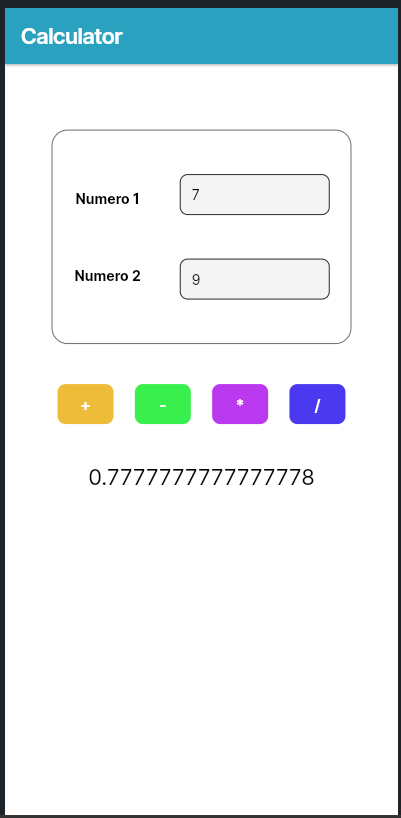
\includegraphics[width=0.25\textwidth]{img/division.png}
  \caption{Resultado de la división: $7 \div 9 \approx 0.7778$}
  \label{fig:division}
\end{figure}
\newpage
\subsection{Evaluación de Componentes}

La tabla~\ref{tab:resultados} resume el estado de implementación de cada componente clave de la calculadora.

\begin{table}[H]
\centering
\caption{Estado de implementación de componentes de la calculadora}
\label{tab:resultados}
\renewcommand{\arraystretch}{1.4}
\begin{tabular}{>{\bfseries}p{5.0cm} p{4.0cm} p{4.0cm}}
\toprule
Componente & Estado & Funcionalidad \\
\midrule
Campos de entrada numéricos & \checkmark\ Implementado & Captura valores correctamente \\
Botones de operación & \checkmark\ Implementado & 4 operaciones disponibles \\
Variable de estado \texttt{result} & \checkmark\ Funcional & Almacena y actualiza resultados \\
Action Flow Editor & \checkmark\ Configurado & Flujos para cada operación \\
Inline Functions & \checkmark\ Implementado & Cálculos matemáticos precisos \\
Widget de visualización & \checkmark\ Reactivo & Actualización automática \\
\bottomrule
\end{tabular}
\end{table}

\subsection{Observaciones Técnicas}

Durante el desarrollo se identificaron los siguientes aspectos relevantes:

\begin{enumerate}
  \item \textbf{Actualización reactiva}: el widget \texttt{Text} vinculado a la variable \texttt{result} se actualiza automáticamente sin necesidad de código adicional, demostrando la naturaleza reactiva de FlutterFlow.

  \item \textbf{Precisión decimal}: la división retorna valores de tipo \texttt{Double} con precisión decimal completa ($7 \div 9 = 0.777777\ldots$), lo que confirma el correcto tipado de la variable de estado.

  \item \textbf{Reutilización de flujos}: aunque cada botón tiene su propio \textit{Action Flow}, la estructura es idéntica en todos los casos, variando únicamente el operador matemático en la \textit{Inline Function}.

  \item \textbf{Validación de entrada}: los campos \texttt{TextField} configurados con \texttt{Keyboard Type: Number} previenen automáticamente la entrada de caracteres no numéricos, mejorando la robustez de la aplicación.
\end{enumerate}

% ============================================================
%  6. CONCLUSIONES
% ============================================================
\section{Conclusiones}

\begin{enumerate}
  \item FlutterFlow permite desarrollar aplicaciones Flutter funcionales sin escribir código manualmente, mediante la combinación de componentes visuales (\textit{widgets}), variables de estado y flujos de acciones configurables.

  \item El sistema de \textbf{Page State} de FlutterFlow implementa el patrón reactivo de Flutter, permitiendo que los widgets se actualicen automáticamente cuando las variables a las que están vinculados cambian de valor, sin necesidad de gestionar manualmente la reconstrucción de la interfaz.

  \item El \textbf{Action Flow Editor} proporciona una abstracción visual efectiva para implementar lógica de negocio, estructurando las operaciones en flujos secuenciales de acciones comprensibles sin necesidad de leer código Dart.

  \item Las \textbf{Inline Functions} permiten integrar código Dart personalizado en puntos específicos del flujo, ofreciendo flexibilidad cuando la configuración visual no es suficiente, sin romper el flujo de trabajo visual predominante.

  \item La configuración de tipos de datos en los componentes (\texttt{Number} para \textit{TextFields}, \texttt{Double} para variables de estado) demuestra que FlutterFlow mantiene la seguridad de tipos característica de Dart, evitando errores en tiempo de ejecución.

  \item El desarrollo de la calculadora evidencia que las plataformas \textit{low-code} como FlutterFlow son apropiadas no solo para aplicaciones de visualización de datos, sino también para implementar lógica computacional, manejo de estado y flujos de interacción complejos.
\end{enumerate}

% ============================================================
%  7. RECOMENDACIONES
% ============================================================
\section{Recomendaciones}

\begin{enumerate}
  \item \textbf{Planificar la estructura de variables de estado antes de implementar la interfaz.} Definir anticipadamente qué datos serán de ámbito \textit{App State} (globales) y cuáles de \textit{Page State} (locales) facilita el diseño de flujos de acciones y evita refactorizaciones posteriores.

  \item \textbf{Utilizar nombres descriptivos para variables y componentes.} FlutterFlow genera referencias automáticas basadas en los nombres asignados (\texttt{inputNum1}, \texttt{result}, etc.); nombres claros mejoran la legibilidad de los \textit{Action Flows} y facilitan el mantenimiento.

  \item \textbf{Aprovechar la validación de tipos en TextFields.} Configurar el \texttt{Keyboard Type} apropiado (\textit{Number}, \textit{Email}, \textit{Phone}) no solo mejora la experiencia de usuario, sino que previene errores de tipo en tiempo de ejecución al procesar los datos.

  \item \textbf{Documentar las Inline Functions con comentarios.} Aunque FlutterFlow es visual, las expresiones de código Dart dentro de \textit{Inline Functions} deben incluir comentarios explicativos cuando implementen lógica no trivial, facilitando la comprensión al exportar el proyecto.

  \item \textbf{Probar los Action Flows con el modo de vista previa (\textit{Preview Mode}).} FlutterFlow permite ejecutar la aplicación en tiempo real dentro del editor; utilizar esta funcionalidad reduce el tiempo de iteración al validar flujos de acciones sin necesidad de compilar.

  \item \textbf{Considerar el manejo de errores en operaciones matemáticas.} Aunque la calculadora actual funciona correctamente con entradas válidas, implementar validaciones para casos límite (división por cero, campos vacíos, valores muy grandes) mediante condiciones en el \textit{Action Flow} mejoraría la robustez de la aplicación.

  \item \textbf{Explorar la exportación de código Flutter.} FlutterFlow permite descargar el proyecto como código Dart/Flutter estándar; revisar el código generado es una excelente oportunidad de aprendizaje para comprender cómo la configuración visual se traduce a código programático.

  \item \textbf{Utilizar componentes reutilizables (\textit{Custom Widgets}) para interfaces repetitivas.} Si la aplicación creciera con más funcionalidades (calculadora científica, conversiones de unidades, etc.), encapsular grupos de widgets en componentes personalizados facilitaría el mantenimiento y la consistencia visual.
\end{enumerate}

% ============================================================
%  REFERENCIAS
% ============================================================
\newpage
\addcontentsline{toc}{section}{Referencias}
\begin{thebibliography}{9}

\bibitem{flutterflow2024}
FlutterFlow Inc. (2024). \textit{FlutterFlow Documentation -- Build apps visually}.
Recuperado de \url{https://docs.flutterflow.io/}

\bibitem{flutter2024}
Google LLC. (2024). \textit{Flutter -- Build apps for any screen}. Flutter Documentation.
Recuperado de \url{https://flutter.dev/docs}

\bibitem{lowcode2023}
Sahay, A., Indamutsa, A., Di Ruscio, D., \& Pierantonio, A. (2023). \textit{Supporting the collaborative development of low-code applications}.
In Proceedings of the ACM/IEEE 26th International Conference on Model Driven Engineering Languages and Systems.

\bibitem{gartner2023}
Gartner, Inc. (2023). \textit{Magic Quadrant for Enterprise Low-Code Application Platforms}.
Gartner Research. Recuperado de \url{https://www.gartner.com/en/documents/4530099}

\bibitem{dart2024}
Google LLC. (2024). \textit{Dart programming language -- Overview}. Dart Documentation.
Recuperado de \url{https://dart.dev/overview}

\bibitem{richardson2020}
Richardson, C., \& Rymer, J. R. (2020). \textit{The Forrester Wave: Low-Code Development Platforms For Professional Developers, Q1 2020}.
Forrester Research.

\bibitem{windmill2020}
Windmill, E. (2020). \textit{Flutter in Action}. Manning Publications.
ISBN: 978-1-61729-571-8.

\bibitem{statista2024}
Statista Research. (2024). \textit{Low-code development platform market revenue worldwide}.
Recuperado de \url{https://www.statista.com/statistics/1224895/low-code-platform-market-revenue/}

\end{thebibliography}

% ============================================================
%  ANEXOS
% ============================================================
\newpage
\section*{Anexos}
\addcontentsline{toc}{section}{Anexos}

\noindent
\begin{minipage}[t]{0.47\textwidth}
  \centering
  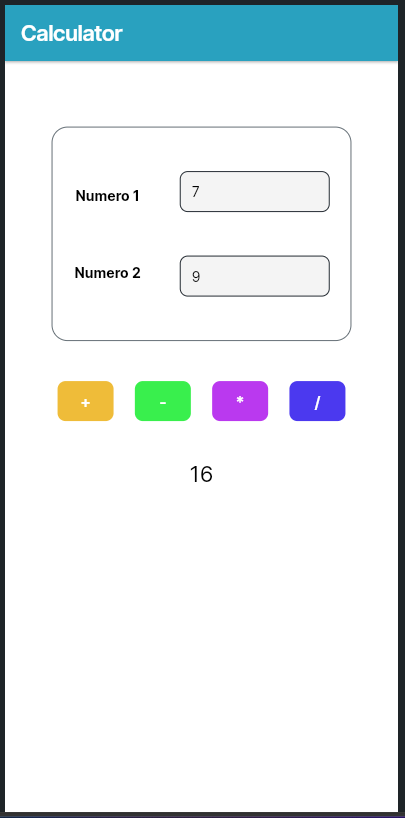
\includegraphics[width=\linewidth]{img/suma.png}
  \captionof{anexofloat}{Operación de suma: $7 + 9 = 16$}
\end{minipage}
\hfill
\begin{minipage}[t]{0.47\textwidth}
  \centering
  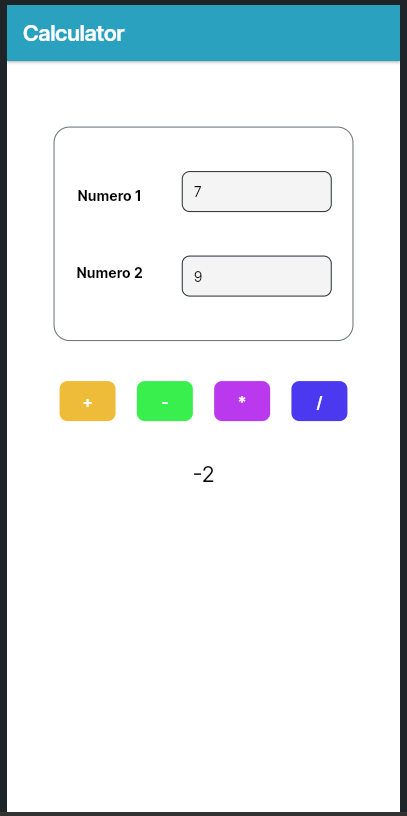
\includegraphics[width=\linewidth]{img/resta.png}
  \captionof{anexofloat}{Operación de resta: $7 - 9 = -2$}
\end{minipage}

\vspace{1.2cm}

\noindent
\begin{minipage}[t]{0.47\textwidth}
  \centering
  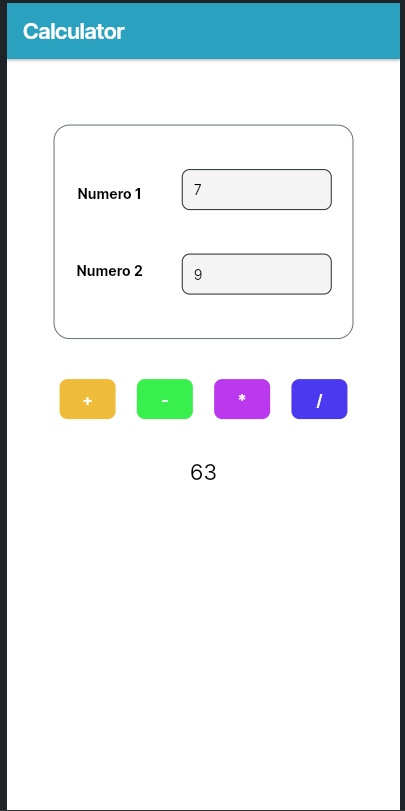
\includegraphics[width=\linewidth]{img/multiplicacion.png}
  \captionof{anexofloat}{Operación de multiplicación: $7 \times 9 = 63$}
\end{minipage}
\hfill
\begin{minipage}[t]{0.47\textwidth}
  \centering
  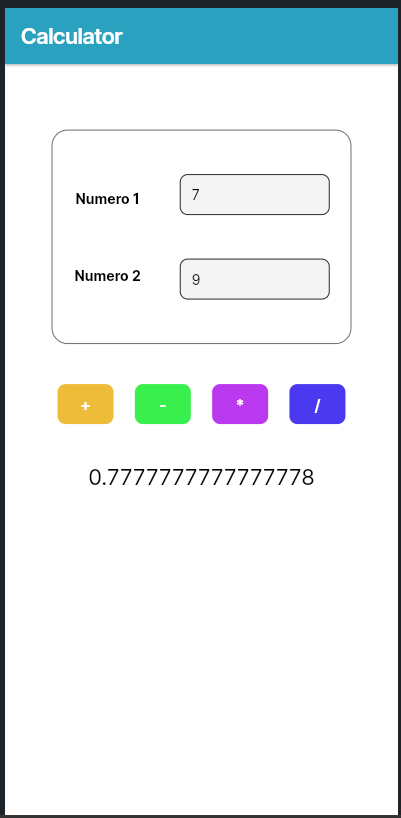
\includegraphics[width=\linewidth]{img/division.png}
  \captionof{anexofloat}{Operación de división: $7 \div 9 \approx 0.7778$}
\end{minipage}

\end{document}
